\chapter{Rhythm}
\vspace{10mm}


\begin{quote}
  {\it   
  ``Compositional activity proves meaningless in the
  absence of a corresponding bodily gestalt.''} --- Ellington's Law 
by Warren Burt 
\end{quote}

\begin{quote}
  {\it ``Jazz without the beat, most musicians know, is a telephone yanked
  from the wall, it just can't communicate.''} --- Leonard Feather,
British author and jazz enthusiast.
\end{quote}

\vspace{7mm}
\section{Understanding Rhythm Through Modeling}
\vspace{5mm}

A fundamental assumption in this work is that representation and modeling
are ways to understand complex real-world processes, in particular, 
the activity of human perception of rhythm. Theories can then be
formulated and verified using empirical data and models, which in 
turn can be updated to reflect new knowledge.  Thus, modeling the cognitive 
processes associated with rhythm and music in general, can yield better
understanding of the functions underlying specific behavioral
responses to music and rhythm.  This knowledge is potentially useful 
to composers, performers, designers of codec\footnote{The term codec 
stands for ``compression/decompression''. A codec is an algorithm, or
specialized computer program that does exactly that. Popular audio
codecs include MPEG 1 Layer 3 (mp3) and Sony minidisc.} 
algorithms, interactive music and media systems \cite{Desain:92}.
These models embody functional relationships between physical
properties of sound and resulting human behavior and sensations.
Thus it is important to make distinctions between the physical
properties of sound, called {\it phenomenal}, that can be measured and their
perceptual correlates.  
%
% looks good as is
%\begin{center}
%
\begin{table}
\begin{tabular}{|l|l|} % all cell contents aligned center
 \hline 
 & \\
 Physical properties of sound  & Perceptual correlates \\ \hline \hline
 & \\
 Frequency & Pitch   \\ \hline
 & \\
 Signal Intensity & Loudness   \\ \hline
 & \\
 Differences in sounds with identical loudness and pitch & Timbre \\ \hline
\end{tabular}
\caption {Properties of sound and their perceptual correlates}
\end{table}
%\end{center}

\vspace{7mm}
\section{Time}
\vspace{3mm}

\subsection{Temporal Representations in Music}

Music is time-based art form that always occurs in some cultural
context. Accordingly, the representation of musical time is 
culturally dependent. Different cultures have time represented 
differently in their cognitive structures, for example, in some 
contexts, time is seen as a circular structure, rather than a
continuum \cite{Gardenfors:2000}. Musical enculturation is thus a 
combination of perception and the organisation of sounds based on 
internalised cultural templates \cite[p. 5]{Smith:99}. Different areas
of research also have different perspectives and interests in
representing time. For example, while musicologists might be
interested in representations that facilitate notation and transcription,
composers and performers might be more interested in representations that 
are designed to work in process-oriented real-time systems \cite{Honing:93}.

There are several different views of temporal representation in
music. These include {\it tacit}, {\it implicit} and {\it explicit}
time. Tacit time frameworks do not represent temporal evolution; there is 
only an idea of ``now''. Implicit time structures employ no definitive 
time relations since time is represented as an absolute, e.g. note
lists, while explicit time structures represent time as relations that
can be compounded to form higher level notions of time. Other
questions that come up in the time modeling process deal with absolute
versus relative time bases, discrete versus continuous representations
and point-based versus intervallic time primitives. Point-based
implies that events are duration-less and occur serially while
intervallic refers to differences between events that form the basis
for meaningful relations (intervals that occur before, after, during) \cite{Honing:93}.

\begin{table}
\begin{tabular}{|l|l|}\hline % | is used for a vertical line
& \\
Low Level: Expression  & {\it Perceptually represented} as departures \\
                       & from canonical proportional values; poorly \\
                       & quantified, and experienced as expressive \\ 
                       & rather than durational effects. \\ 
                       &  \\
                       & {\it In Performance}, represented as programmed\\
                       & variations in the rate of the clock controlling\\
                       & beat durations (see level 2), and as modifications\\
                       & of the procedures specifying individual notes\\
                       & \\ \hline
                       & \\

Middle Level: Rhythm   & {\it Perceptually represented} as collection \\
and meter              & of grouped durational equalities and \\
                       & inequalities organized around a metrical \\
                       & framework (when the music has a meter) \\
                       &  \\
                       & {\it In Performance}, represented as a \\
                       & collection of untimed procedures, organized \\
                       & metrical markers which are directly timed by \\
                       & a programmable clock. \\
                       & \\ \hline
                       &  \\

High Level: Form       & {\it Perceptually represented} as a structure\\
                       & of hierarchical relations, constructed by means\\
                       & of memory processes and perception, and \\
                       & distinguished from level 2 structures by \\
                       & exceeding the length of the perceptual present \\
                       &  \\
                       & {\it In Performance}, represented as a hierarchical \\
                       & memory structure that forms the highest levels\\
                       & of a motor program \\
                       & \\ \hline
\end{tabular}
\caption {A summary of structural levels in musical time based on
  meter and their cognitive/perceptual properties \cite[p. 233]{Clarke:87}.}
\end{table}

\vspace{5mm}
\subsection{Causal versus Non-Causal Analysis}
A further point regarding time arises when an interpretive process must
examine some data structured in time. Some theories propose digesting
whole chunks of data as a unit while others choose to process
the data sequentially in time or causally. Opponents of the former
process, claim that ``theories that behave symmetric with respect to 
time have to be wrong on that basis alone. ... [those] theories 
tend to model the perceiver more like a musicologist studying the
score, instead of a first time listener'' \cite{Desain:92}. On the
other hand, proponents claim that the non-causality of such models
embodies a certain amount of enculturated knowledge that is essential to
any interpretation, citing that performers have spent time with their
music and have definite intentions before a show \cite[p. 55]{Smith:99}. 

Analytically, causal methods can be seen as a subset of the larger
non-causal methods, even though the tools may not be related.
In any case, because humans infer musical structure based on
both universal ``hard-wired'' low level processing of sensory data
(bottom-up processing) {\it and} culture specific knowledge,
expectations and predictions (top-down processing)
\cite[p. 27]{Todd:94}, robust models of rhythm perception must account 
for both bottom-up and top-down processing and cross-cultural variances. 
This makes room for multiple interpretations in which both causal and
non-causal methods are useful.


\begin{table}
\begin{tabular}{|l|l|}\hline % | is used for a vertical line
& \\
0 to 2-5 msecs apart   & Beats are perceived as simultaneous, \\
                       & indistinguishable (even with different \\
                       & loudness, but same duration) as a single\\
                       & event. \\
                       & \\ \hline
                       & \\

2-5 to 40 msecs apart  & Beats are distinguishable, but no order \\
                       & relation can be indicated. \\
                       & \\ \hline
                       &  \\

30 to 50 msecs apart   & Beats above this can produce an order \\
                       & relation. \\
                       & \\ \hline
\end{tabular}
\caption {A table summarising Leigh Smith's review of P{\"o}ppel's
 taxonomy of elementary time experiences \cite[p. 14]{Smith:99} }
\end{table}

\vspace{5mm}
\subsection{Specious Present and Auditory Stores}

Another aspect of time deals with the interval in which
events are processed -- the {\it specious} present. Later called the 
psychological, perceptual or subjective present, it is related to the 
duration within which one experiences a sequence of events as
simultaneously present in consciousness \cite[p. 97]{Gabrielsson:89}\cite{Fraisse:63}.
Parncutt defines this perceptual present as a ``continuous time
interval comprising all real-time percepts and sensations
simultaneously available to attention, perception and cognitive 
processing'' \cite[p. 451]{Parncutt:94}\cite[p. 12]{Smith:99}.

Enabling this present is {\it echoic} memory, a kind of auditory
sensory memory possessing a high degree of structure and organization \cite[p. 451]{Parncutt:94}. 
Echoic memory which is acoustic should be differentiated from {\it iconic} memory which 
is visual. There have been many different estimates in the literature 
on the size of echoic memory and the ``integrating buffers'', most of 
them limiting the echoic memory to less than 500 msec and the
subjective present to 4 seconds, with experimental results ranging 
between 2 and 10 seconds \cite[p. 12-3]{Smith:99}
\cite[p. 451]{Parncutt:94}. Parncutt stresses that because the
``present is so highly adaptive, no fixed parameter values can be
expected to describe it adequately'' \cite[p. 451-2]{Parncutt:94}. 
Furthermore, the present also depends on the rate events occur and 
their complexity and structure \cite[p. 452]{Parncutt:94}.

\vspace{5mm}
\subsection{Synchronisation}

Synchronisation is another aspect of rhythm that emerges from a notion of
time. Mari Riess Jones in an article entitled ``Time, Our Lost
Dimension: Toward a New Theory of Perception, Attention and
Memory'' states that the ``human system in general and the perceptual
system in particular depend upon the properties of endogenous
rhythmic processes in the nervous system'' \cite{Jones:76}. Additionally, 
many studies have suggested the presence of internal clocks and have
noted the strong connection between physical actions and perception 
\cite[p. 17]{Smith:99}. In reaction to a sound stream, humans are able
to forecast and coordinate motor action to coincide with future events
from the sound stream. Smith claims that regularity is less important 
to the act of synchronisation than the listener's expectations and ability to
predict, since accelerating and decelerating rhythms can be
timed \cite{Smith:99}. Jones suggests that parts of the synchronisation process are
based on temporal expectancy.  Thus relations between certain 
time differences (time deltas) will hold for subsequent ones. This allows
the listener to extrapolate time trajectories that predict when events
will occur \cite{Jones:76}. 

\vspace{7mm}
\section{Definitions}
\vspace{3mm}

How should we define rhythm?  Smith reports a variety of responses from the literature
\cite[p. 9-10]{Smith:99}. Eric Clarke used the term broadly to apply
to ``regular, periodic features of the temporal structure of music and
to aperiodic features'' \cite{Clarke:85structure}. Dowling states that
rhythm is a temporally extended pattern of durational and accentual 
relationships, while Parncutt claims that musical rhythm is an
acoustic sequence evoking a sensation of pulse
\cite[p. 451]{Parncutt:94}.  Scheirer cites Handel's claims that
``the experience of rhythm involves movement, regularity, grouping,
and yet accentuation and differentiation'' \cite{Scheirer:98tempo}.

According to psychological studies done by Gabrielsson on human 
``subjects'', rhythm like timbre is a multi-dimensional quality. 
From the empirical studies, Gabrielsson points out the existence of at 
least fifteen dimensions which ``lend themselves to grouping into 
three categories'' related to structural, motional and emotional
aspects of rhythm. Refer to Table 4.

\begin{table}
\begin{tabular}{|l|l|}\hline % | is used for a vertical line
& \\
Structural Aspects     & Meter, position and strength of accents, \\
                       & type and prominence of basic pattern, number \\
                       & of different kinds of subdivisions within \\
                       & beats, uniformity versus variation and  \\
                       & simplicity versus complexity \\
                       & \\ \hline
                       & \\

Motional Aspects       & Tempo and overall rapidity, however motional \\
                       & characters exist such as walking, dancing,  \\
                       & jumping, rocking, swinging, graceful and driving \\
                       & forward \\
                       & \\ \hline
                       &  \\

Emotional Aspects      & Vitality versus dullness, excitement versus \\
                       & calmness, rigidity versus flexibility and  \\
                       & solemnity versus playfulness \\
                       & \\ \hline
\end{tabular}
\caption {Gabrielsson's dimensional categories for rhythm \cite[p. 107]{Gabrielsson:89}}
\end{table}

There are problems in modeling the ``dimensions'' mentioned above
because the interpretive ambiguity of the dimensions and characters 
do not lend easily to symbolic or quantitative representation. 


\vspace{7mm}
\section{Pulse}
\vspace{3mm}

Parncutt's definition of a musical rhythm is an acoustic
sequence evoking a sensation of pulse.  How should we define pulse?  
If a car drives by loudly broadcasting music, in the several seconds within
which the music is in earshot, the pulse would be the subjective
evaluation of the feel or impression of movement inferred from the
music. If that music happened to be tabla drumming, Olatunji, Faithless or
Subotnick, each would leave a different but firm impression in the mind
of the listener.  
The percept of pulse is confined to the time interval called the
subjective present \cite[p. 451]{Parncutt:94}. While {\it rhythm}
deals with grouping and time hierarchies and {\it tempo} involves the 
rate at which rhythmically significant events occur, pulse corresponds
to a ``sense of equally spaced phenomenal impulses''
\cite{Scheirer:98tempo}. For many kinds of music, the pulse is the
``foot-tapping'' beat.

Pulse has also gone by other names like {\it tactus}, defined by Lerdahl and
Jackendoff to describe the most salient hierarchical level at which
the listener will tap their foot in accompaniment to a rhythm \cite[p. 31]{Smith:99}.
Parncutt defines it as a trivial sense of expectancy. Once a pulse is
established, subsequent events are ``expected'' with some time
trajectory. This is of course related to our discussion above of
synchronisation, where motor actions move along time trajectories
inferred from this expectation \cite[p. 453]{Parncutt:94}.

\vspace{5mm}
\subsection{Pulse Outside A Metrical Context}

In non-metric musics, the pulse may not necessarily correspond to an
isochronous period.  Researchers agree that the idea of a basic pulse
in such music is ``usually misplaced'' \cite[p. 190]{Magill:97}
Magill reports that 
\begin{quote}
``West African drum ensemble music takes a multilayered approach to
rhythm, with all the parts being related to a fundamental {\it time
line}, often played on a bell... Bell patterns can nearly always be
subdivided into a number of regular pulses (usually 8, 12, or
16). Time lines or bell patterns betray asymmetric construction
and sound syncopated to Western ears'' \cite[p. 190]{Magill:97}.
\end{quote}

For example, in the A{\it n}lo drumming style from southern Ghana, 
Pantaleoni points out that it is ``the bell that regulates the play, 
and not the steady pulse some player or observer might feel, because 
the bell can put each pattern into its proper places, while a simple
pulse can only regulate the speed with which the pattern is played''
\cite[p. 60]{Pantaleoni:72}. Magill states that in many West African 
drumming styles while some instruments reinforce an underlying fast pulse, 
others might highlight portions of a bell pattern while others provide
a complex overlay of rhythms and meters \cite[p. 190]{Magill:97}. In
any case, while regular pulses are quite common, the traditional 
cultural view is that they are of peripheral importance compared 
to the asymmetric time line. The definition of pulse needs to be 
revised to be a periodic structuring or synchronization framework, 
since in the kinds of music discussed above, asymmetric time lines 
and isochronous pulses are both constructs within which higher levels 
of rhythmic time are structured. 

\vspace{5mm}
\subsubsection{ The Fastest Pulse }

Attempts to understand non-metric music have also emerged in the form of
concepts like the ``fastest pulse''. The fastest pulse is defined as 
the ``beat with the shortest duration in the music considered''
\cite[p. 33]{Smith:99} Smith cites Koetting's warning that the fastest
pulse does not seem to describe how African timing is perceived
\cite[p. 33]{Smith:99}.  Pantaleoni comments \begin{quote} ``I have
not found it to be a concept familiar to those African drummer with 
whom I have worked, nor does it seem to be an easy concept for them to
use once it has been explained. Perhaps it is simply difficult for a 
performer to think as an analyst, but in the absence of some kind of 
positive support from the musicians themselves it cannot be assumed 
that a convenient analytical tool corresponds to the basic pulse or 
principle of timing which actually functions in the playing of the 
music'' \cite[p. 58]{Pantaleoni:72}. \end{quote}
While clearly limited from a compositional and improvisational point 
of view, the idea of the fastest pulse might still be useful in
analysis. As will be seen in the next chapter, analyses that determine
the fastest pulse, per extracted stream, are a useful interpretive tool.

\vspace{5mm}
\subsection{Beat Induction}

Beat induction is a synchronization process with a phenomenal pulse.  
There have been many successful attempts to measure the pulse 
computationally in Western classical and popular music, using that 
information to drive a foot-tapping process.  
Eric Scheirer used filterbanks and parallel comb filters to extract
amplitude envelopes and infer the beat from arbitrarily complex 
musical signals \cite{Scheirer:98tempo}.  Povel and Essens introduced 
the idea of ``internal clocks'' which are selected based on a set of 
inter-onset interval inputs. Desain and Honing have several computational beat-tracking 
methods to their name. Given an onset stream, their models 
return the beat of the stream. Different from the 
previous methods, Desain and Honing use a causal process model which takes the
onset inputs sequentially and updates an expectancy measure.  The
beat is then inferred from regions of high expectancy. Large and Kolen's
beat-tracking model is based on non-linear oscillators. From a stream
of onsets, a ``gradient-descent method'' is employed to continually
update the period and phase of an oscillator, which represents the
pulse \cite{Large:94}\cite{Scheirer:98tempo}. Goto presented a system 
which ``combines both low-level ``bottom-up'' signal processing and 
high-level pattern matching and ``agent-based'' representation to 
beat-track and do simple rhythmic grouping for popular music''
\cite{Scheirer:98tempo}\cite{Goto:98}. Leigh Smith has also explored a
multiscale representation of musical rhythm. Onset streams or pulse
trains are first decomposed using a Morlet wavelet basis. The
``foot-tapping'' pulse of a section of music is then extracted by 
correlating frequency modulation ridges extracted from the wavelet
decomposition using stationary phase, modulus maxima, dilation scale 
derivatives and local phase congruency. Refer to \cite{Smith:99} for 
definitions and implementation details.

\vspace{5mm}
\subsection{Tempo}
Tempo is defined here as the rate at which rhythmically significant
events occur. In music with an isochronous pulse, tempo is the rate of
the tactus. In much Western music and popular music, this is the ``foot
tapping'' rate. In non-metrical settings, there may not be any explicit
overall tempo. In this case, there may be multiple rhythmic layers
each with its own individual rate. Tempo is however best used in a 
metrical setting. Commercial software systems express tempo in terms 
of beats per minute (BPM), while numerous scores have subjective tempo 
indications like {\it Larghissimo} or {\it Prestissimo} or more
concrete markings like quarter note equals sixty.

Within the above framework how do variations in tempo affect the
interpretation of rhythmic structure?  Clarke reports that slow tempi
aid the cognitive process of segmentation at structural boundary
points while at higher tempi, music tends to be grouped into fewer
units. This is claimed to occur because of the limits of the subjective
present. In other words, at faster tempi, more elements are packed into
the subjective present; thus given fixed maximum neural processing
rates, music is subdivided into larger groups in accordance with 
its structural properties \cite[p. 36]{Smith:99}.

\vspace{7mm}
\section{Grouping}
\vspace{3mm}

Experiencing rhythm occurs as a whole sequence or pattern, not as
individual events. Within the subjective present, how a sequence 
is formed by segregating a stream of events is called grouping. This
can take the form of phrases or motives. In many cases, the number of 
events grouped together depends on the presentation
rate, so the faster the rate, the more members are included in the
group. This extends up to perceptual limits.  Some rhythmic 
groups are presented so quickly that they're not perceived as
individual rhythms or events but are lumped together to form a pitch percept. 
Within a sequence of events, certain ones with objective accents or 
differences suggest or confirm the presence of a perceptual group
boundary.  Quantities responsible for the percept of a group 
boundary include perceptual limits on memory and attention and 
cognitive representations.

Smith points out two principal grouping principles: The {\it run} 
principle and the {\it gap} principle.  The run principle proposes that 
the longest run of similar events will begin a rhythmic pattern. 
Listeners tend to group sounds of the same intensity together. Runs of 
different intensity will be organized so that the longest runs are
placed at the beginning or end of the pattern, never in the middle. 
The gap principle refers to boundaries that are formed between 
dissimilar elements. Rests partition elements while elements close 
in time tend to be grouped \cite[p. 28]{Smith:99}. These principles
are based on Gestalt principles of perceptual organization and
Bregman's seminal work on auditory scene analysis
\cite{Bregman:90}. Additionally, higher level grouping structures are 
bounded by repetitions. A single change in an established pattern 
can affect the entire grouping percept \cite[p. 28]{Smith:99}.

Parncutt defines two independent kinds of temporal grouping, 
{\it serial} and {\it periodic}. Serial grouping (related to the gap
principle) is dependent on the serial proximity of adjacent events in
time, pitch and timbre. ``According to Lerdahl and Jackendoff (1983), 
serial grouping in music includes ``motives, themes, phrases, periods,
theme-groups, sections, and the piece itself'' \cite{Lerdahl:83}. 
Periodic grouping on other hand, depends on the relative times and 
perceptual properties of {\it nonadjacent} events \cite[p. 412]{Parncutt:94}.

\vspace{5mm}
\subsection{Meter}

Meter can be seen as a form of periodic grouping. Parncutt states that it
groups events into equivalence classes, such as all {\it n}th beats of
a bar \cite[p. 412]{Parncutt:94}. He further classifies periodic
grouping as being an aggregate of two stages, {\it pulse sensation} and
{\it perceived meter}. Interestingly enough, Halsband conversely
states that grouping ``plays a major role in the perception of all metrically
organized music'' \cite[p. 266]{Halsband:94}.  

While grouping is a psychological term, meter is a product of music
theory and associated forms of notation. Repetition in meter, as in 
other groupings, plays an integral role in the determination 
of a metrical percept. However, the perceived meter in a performance 
may not necessarily correspond to the notated meter. In many of these 
cases, some initial metrical orientation influences the interpretation
of subsequent sequences.  

There are rarely explicit rules to outline an interpretation; in 
improvisational styles, performances ``unbounded by a strict
metric frame are not free in the sense of being unrhythmic. Rather, 
they are driven by rhythmic goals that are elastic'' \cite[p. 158]{Berliner:94}.

Handel showed empirically that difficult rhythms with atypical
metrical accenting were perceived in terms of elemental grouping
schemes, rather than as a meter with a timing interval \cite[p. 31]{Smith:99}.
Thus, a metrical percept is a regular alternation of strong and weak
beats. What then qualifies an event as particularly strong or weak?

\begin{table}
\begin{tabular}{|l|l|}\hline % | is used for a vertical line
& \\
Well-Formedness Rule 1 & Every attack point must be associated with \\
                       & a beat at the smallest level metrical level \\
                       & present at that point in the piece. \\
                       & \\ \hline
                       & \\

Well-Formedness Rule 2 & Every beat at a given level must also be a \\
                       & beat at all smaller levels present at that \\
                       & point in the piece. \\
                       & \\ \hline
                       & \\

Well-Formedness Rule 3 & At each metrical level, strong beats are \\ 
                       & spaced either two or three beats apart. \\
                       & \\ \hline
                       &  \\

Well-Formedness Rule 4 & The tactus and immediately larger metrical \\
                       & levels must consist of beats equally spaced \\
                       & throughout the piece. At subtactus metrical  \\ 
                       & levels, weak beats must be equally spaced \\
                       & between surrounding strong beats. \\
                       & \\ \hline
\end{tabular}
\caption {A summary of Lerdahl and Jackendoff's Metrical Well-Formedness
  Rules from their ``Generative Theory of Tonal Music'' \cite{Lerdahl:83}.}
\end{table}

\vspace{5mm}
\subsection{Accentuation}

Accents are differences in adjacent events that separate them and suggest 
particular grouping configurations. Smith cites Lerhdahl and
Jackendoff as distinguishing three kinds of accents, {\it phenomenal},
{\it metrical} and {\it structural} according to their effect on 
groups \cite[p. 19]{Smith:99}. Phenomenal accents are said
to exist superficially, stressing a single moment and enabling
syncopations. Metrical accents occur when the emphasised beat is
part of a repeating metrical pattern. Structural accents occur at
points hierarchically higher than meter. For example, structural accents 
could delimit phrases or sections.  Furthermore, a ``phenomenal accent
functions as a perceptual input to metrical accent'' \cite{Lerdahl:83}.

Accents occur when there are changes in duration, inter-onset 
interval (IOI), pitch, articulation, timbre or combinations thereof. 
Similarly changes in phrase length, time expectancies, event density 
(flams, fills, etc) or multiple event synchronisation can cause
accentuation \cite[p. 19]{Smith:99} \cite[p. 426]{Parncutt:94}. 

Articulation is one way to signify an accent. Berliner remarks that in
the jazz idiom, ghosting ``on-beat pitches in an eight-note sequence
creates de facto accents on every off-beat, increasing rhythmic
tension. Reversing the procedure relieves rhythmic
tension... Similarly the varied application of hard, soft and ghosted
attacks can shift accents within a repeated eight-note triplet, changing
its perceived rhythmic configuration and its relative syncopated
quality'' \cite[p. 156]{Berliner:94}.


\begin{figure}[thp]
  \begin{center}
    \resizebox{5in}{!}{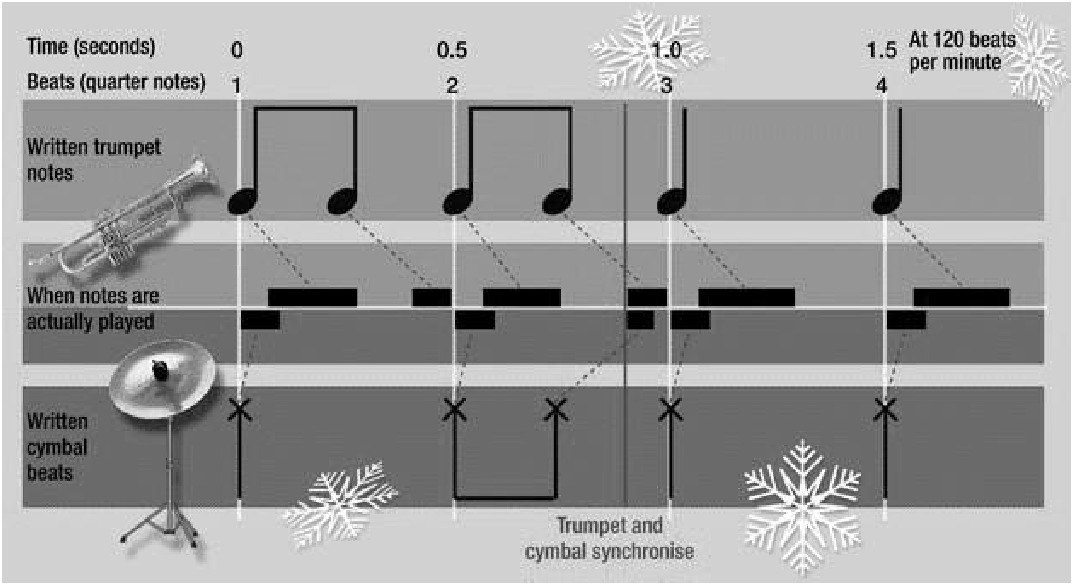
\includegraphics{AllThatJazz.pdf}}
    \caption{``For a swinging performance the first of each pair of
      eight notes is played longer than the second. The melody line
      also hangs behind the cymbal beat, except for the occasional
      off-beat synchronisation, which keeps the band together'' \cite{Hamer:2000}}
    \label{allthatJazz}
  \end{center}
\end{figure}

Accentuation is not always applicable to specifying grouping structure
and its use varies with the musical context. For instance, using the 
A{\it n}lo dance drumming example, Pantaleoni reports that ``variation
in loudness (phenomenal accents) is indeed an important part of the 
character of a rhythmic line in Atsi{\~ a}, but no evidence indicates 
that its contribution is more than melodic... Dynamic stress would
seem to be individual, decorative, incidental, and often illusory, 
hardly a likely clue to rhythmic organisation'' \cite[pp. 54]{Pantaleoni:72}.

\vspace{7mm}
\section{Expressive Timing}
\vspace{3mm}

Many authors have explored what is known in rhythmic performances as
expressive timing. Discrepancies can always be found in the timing
dictated by a score and that which occurs in a performance. Barring
mistakes, which really are not plausible with highly trained musicians
familiar with the music, these deviations are ``related to the
structural properties of the music and to the ways the performers
organize'' these properties \cite{Clarke:85structure}. In an analysis 
of Erik Satie's ``Gnossienne No. 5'', Clarke reports that 
\begin{quote} ``the tempo marking is followed by the instruction ``souple et
expressif''. This is relevant to subsequent analysis, since it
suggests that the performance of the piece should avoid metronomic
tendencies in the left hand, and may encourage a rhythmic flexibility
in the right hand that conventional notation cannot convey'' \cite[p. 300]{Clarke:85}.
\end{quote}

Research has thus focused on determining exactly what deviations from 
the score contribute to a subjective feeling of expression that is 
not ``metronomic''. First some definitions: expressive timing refers 
to deviations in notated times that suggest particular structural 
interpretations or give the temporal development of the music a 
particular feel or sense of movement. Smith cites certain kinds
of expressive timing as having evolved from a performance practice 
known as {\it rubato}, literally ``robbed time''
\cite[pp. 37]{Smith:99}. In computer music, terms like ``micro-tempo''
are used to describe this expressive phenomenon of local tempo
changing from event to event. In all cases,
these expressive timing transformations are used by performers either 
in response to structural features in the score or in attempt to
explore new interpretive configurations  or impose a particular
structure on structurally indeterminate material \cite{Clarke:85structure}.

\begin{figure}[thp]
  \begin{center}
    \resizebox{4.5in}{!}{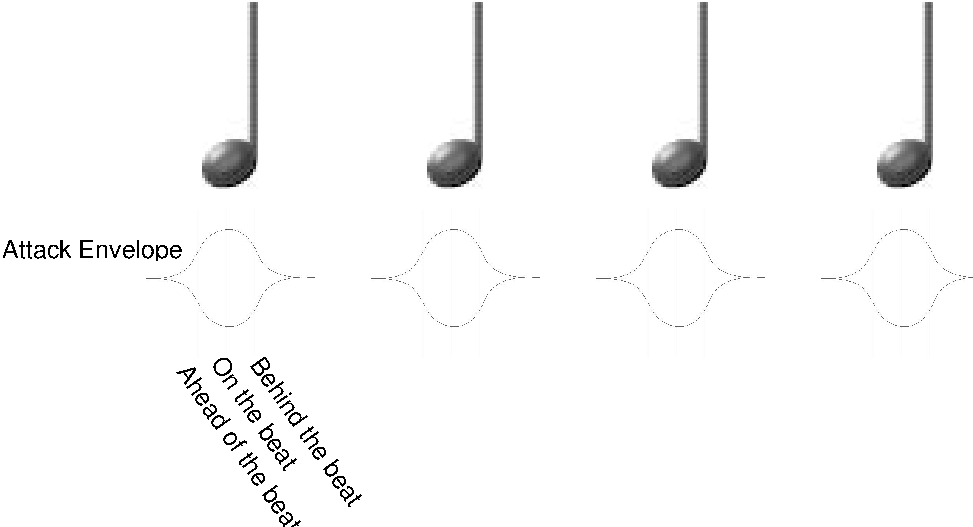
\includegraphics{OnBeat.pdf}}
    \caption{``Imagining the beat as an ``elliptical figure'', the
      drummer or bass player can play either ``ahead of the beat''
      (that is, on the front part of the elliptical figure), ``behind
      the beat'', (that is on the very end of the elliptical figure or
      in varying degrees toward the center of the figure or ``on the
      beat'' (that is, the center of the figure)'' \cite[p. 151]{Berliner:94}.}
    \label{on the beat}
  \end{center}
\end{figure}

In the jazz tradition, Berliner says that musicians ``talk about 
playing on three different parts of the beat without making any
difference in the overall tempo''. On a similar note, Fred Hersch
claims that \begin{quote} ``there should be ten, fifteen different
  kinds of time. There's a kind of time that has an edge on it for a
  while and lays back for a while. Sometimes it rolls over the bar,
  and sometimes it sits more on the beats.  That's what makes it
  interesting. You can set a metronome here and by playing with an
  edge or playing behind it or right in the center you can get all
  kinds of different feelings. That's what makes it come alive. People
  are human, and rhythmic energy has an ebb and flow'' \cite[p. 151]{Berliner:94}. \end{quote}

\vspace{5mm}
\subsection{Tempo Curves}

Tempo curves are one way that timing deviations are represented in
contemporary music software applications for notated music, offering 
a measure of ``beat-by-beat time deviation from a canonical metrical grid'' \cite[p. 39]{Smith:99}.
This quasi-instantaneous tempo or {\it Local tempo} is defined
computationally as the event to event ratio of score time interval
to performance time interval. $$ Local\ tempo = Global \ tempo \times {Score \ time \ interval
  \over Performance \ time \ interval}$$ Tempo curves are thus 
constructed by connecting points with straight line segments between local
tempo measures of each performed note in the score \cite{Smith:99}\cite{Desain:91}.

\vspace{5mm}
\subsection{Expression and Structure}

Desain and Honing warn that while they are useful to study expressive
timing, tempo curves can be is a ``dangerous notion''. This is because
it encourages ``its users into the false impression that it has a musical and
psychological reality. There is no abstract tempo curve in the music
nor is there a mental tempo curve in the head of the performer or
listener'' \cite{Desain:91}. This is because tempo curves by themselves
contain no structural information. Thus global transformations, like 
scaling the overall tempo curve, will change timing relationships 
between notes that are ornamental and {\it invariant} with tempo. 
Furthermore, attempts to impose a tempo curve from the performance of 
one piece onto the score of another shows that tempo curves convey an 
erroneous notion that time is independent of the note events that mark it.
This clearly ignores the fact that the expression captured by the
tempo curve can only function with respect to the original
music performance from which it was derived \cite{Smith:99}\cite{Desain:91}\cite{Desain:91towards}. 

For a more in-depth discussion on expressive temporal transformations,
refer to Desain and Honing's paper called ``Towards a Calculus for 
Expressive Timing in Music'' \cite{Desain:91towards}. 


\vspace{7mm}
\section{A West African Concept of Rhythmic Time}
\vspace{3mm}


\subsection{Misunderstandings...}

The relative lack of serious research on rhythm in sub-saharan 
African music is frankly baffling, given traditions so rich in 
rhythmic textures and structures. The {\sl Journal de la Discotheque 
Internationale de Musique Africaine} and the rare article in {\sl
Music Perception} are the only academic journals where such music 
is even discussed. 

On the one hand, this paucity of work is understandable as most of the 
research in cognitive sciences is being done in Western universities 
with funding from local or national organizations; this is compounded 
by the fact that even the relatively simple rhythmic structure of 
most occidental music is still largely poorly understood.  What is
particularly grievous on the other hand is that the choice of music
chosen for experiments mirrors the aesthetic imperialism present in 
the global music industry. 

Furthermore, within Africa, the majority of research on rhythm
curiously involves Ghanian dance drumming. This in itself is peculiar,
as the Ghanian styles are hardly representative of West 
African music. In many respects, any one of the plethora of cultures 
can hardly represent the varied use of rhythms. Again, I suspect that 
the popularity of such studies is strongly linked to the patronization
of Ghanian music schools by the Western academic elite and well-known
composers like Steve Reich, as well as a much stronger push by
Ghanians to export their culture.

\vspace{5mm}
\subsection{Asymmetric Cognitive Clocks}

One useful research effort that appeared in a recent issue of 
{\sl Music Perception} investigated mental models used by expert 
African drummers in the production of polyrhythmic patterns. The 
paper fits into the category of work which pursues computational 
validation of ``culturally initiated beliefs'' about cognitive 
models. (That cultural aspects of a music and its production would 
not even be considered in a computational model is bewildering.)

Experiments were conducted by recording the performance of 
a master Asante drummer's spontaneous patterns and responses to a
computer generated tone. Quantities such as pulse hand allocation
(left or right), pulse stream size (three or four) were varied and 
measured \cite[p. 191]{Magill:97}.  The goal was to determine if the 
African cultural description of the cognitive process involved in 
producing rhythm is valid by computationally modeling the process 
and experimentally verifying its validity. The performance data was also
run through a pulse-ground(PG) model based on the notion of meter as a 
means to check the data against another well understood model \cite[p. 191]{Magill:97}.

The model used in the experiments is an asymmetric time-line-ground(TLG) model 
that represents a computational elaboration of the multilayered
traditional West African understanding that all instruments 
in a percussion ensemble play in relation to a fundamental {\it time-line}.
The asymmetry of the time-line Magill claims doesn't ``reduce to one of
additive meter'' \cite[p. 191]{Magill:97} because much West African
music is founded on the presence of parallel isochronous pulse streams
that regularly cut across the additive subgroups. This is possible
because the cycle lengths of the asymmetric time-line are composite 
numbers (6, 8, 12, 24).  Furthermore, TLG model ``allows for the
presence of unequal clock pulses but assumes that where clock
intervals are of the same duration, the variance of those two clock
pulses will be equal'' \cite[p. 191]{Magill:97}.

In performances by the master Asante drummer, Magill reports that 
the TLG provides a ``convincing'' fit to seven of the eight tests.
The eighth required some modifications to the basic model. 
Magill comments further that the ``asymmetric process'' need not be
based on the single fastest pulse (additive meter) even though the
experimental results can be viewed in this light.

 


